\chapter{Project}

\section{Code Concept}

\section{Base}
In extend to this article is a code base avaiable \footnote{\url{https://www.github.com/florianwiech/incremental-machine-learning}}.
This code base includes the reimplementation of EWC and the extension of modifying the Fisher Information Matrix.
The concept documents the code structure and procedure.

The complete code consists of three files.
"main.py", "network.py" and "mnist.py".

\begin{figure}[H]
    \centering
    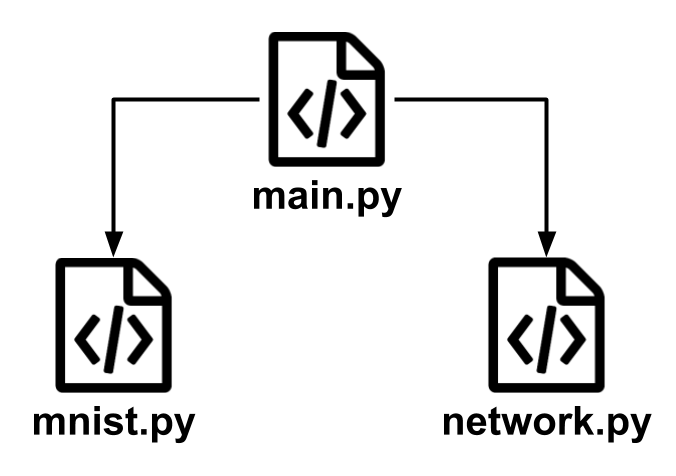
\includegraphics[scale=.4]{project/concept/files}
    \caption{File structure}
    \label{fig:concept_file_structure}
\end{figure}

The "\textbf{mnist.py}" makes the mnist dataset available.
It loads the mnist database automatically, reshapes the values and data structures and splits or permutes the dataset if neccesary.
After the calculation it returns the arrays in Python standard datastructures with the extension of multi-dimensional arrays from NumPy.
\newline
"\textbf{network.py}" holds the "Network" class.
The class consists of all neccesary operations for the EWC algorithm with original and adaption.
The contructor creates a neural network with 784 input neurons, three hidden layers with each 800 neurons and the ten mnist output classes.
In addition to that it initializes all neccesary functions like loss and accuracy.
After initialization the object offers several methods for training, testing and applying EWC to the task.
Figure \ref{fig:concept_class_diagram} shows a class diagram of the Network class.

\begin{figure}[H]
    \centering
    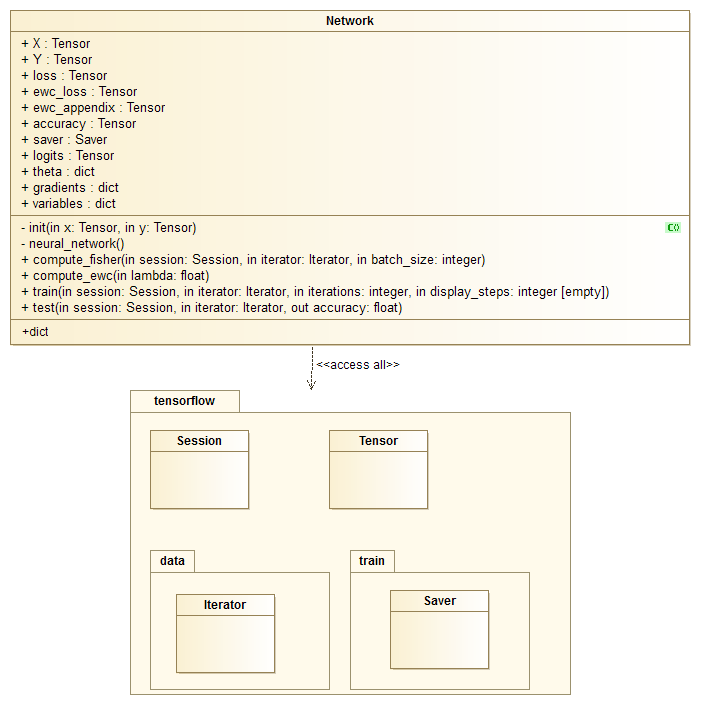
\includegraphics[scale=.6]{project/concept/class_diagram}
    \caption{Class diagram}
    \label{fig:concept_class_diagram}
\end{figure}

While execution the networks occupies multiple states.
The states distinguish if the network trains the first task or loads a previous state and retrains the network.
Figure \ref{fig:concept_state_diagram} shows the state diagram for the network:

\begin{figure}[H]
    \centering
    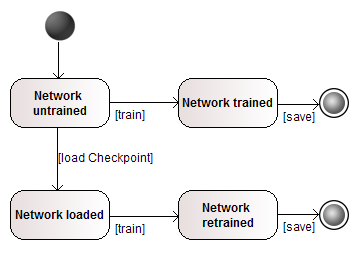
\includegraphics[scale=.8]{project/concept/state_diagram}
    \caption{State diagram}
    \label{fig:concept_state_diagram}
\end{figure}

"\textbf{main.py}" is the entrypoint of the code base.
It offers an command line tool for specification of the neccesary parameters.
\newline
The main function executes one tasks and saves their state in a checkpoint.
The task execution includes loading a checkpoint if it is not the first task or initialize a untrained network.
After that training or retraining the network and calculating the matrix if the new network should be saved.
Then perform an accuracy check on the testset and exit the script.
To train the second task the script has to be started again with different parameters.

The sequential execution is shown in a sequence diagram.
The first part (Figure \ref{fig:concept_sequence_diagram_part_1}) shows the initialization of all neccesary parameter and objects.
Part 2 (Figure \ref{fig:concept_sequence_diagram_part_2}) shows the execution of training and testing the neural network.

\begin{figure}[H]
    \centering
    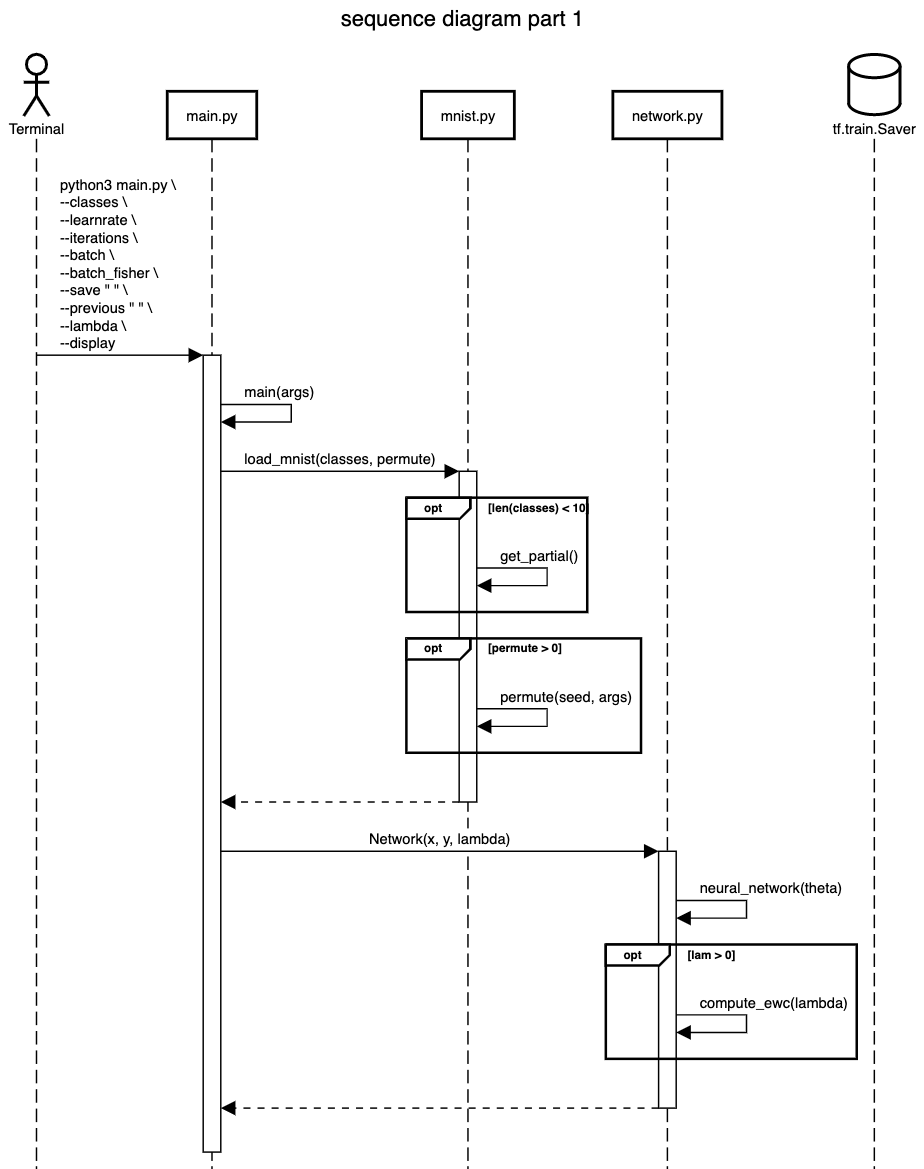
\includegraphics[width=\textwidth]{project/concept/sequence_diagram_part_1}
    \caption{Sequence diagram part 1}
    \label{fig:concept_sequence_diagram_part_1}
\end{figure}

\begin{figure}[H]
    \centering
    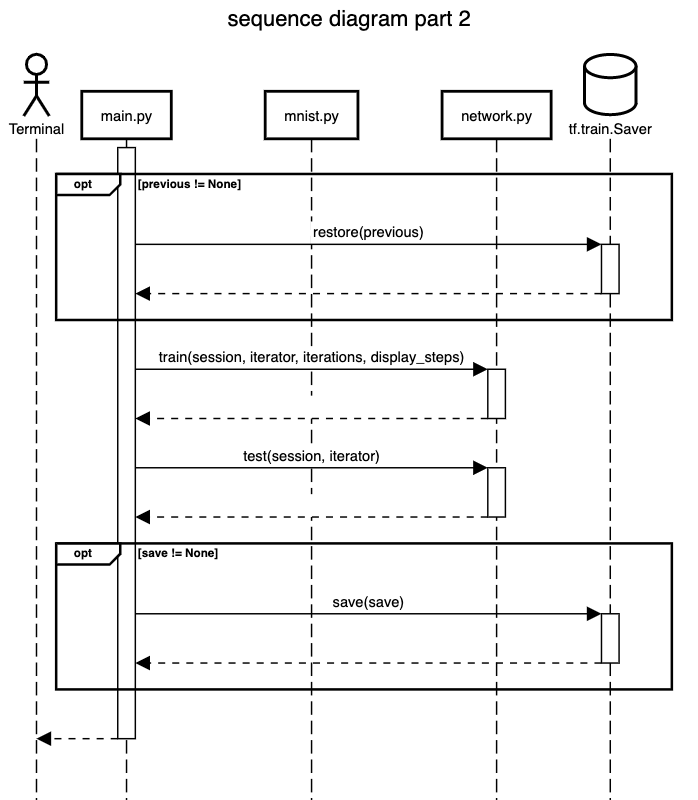
\includegraphics[width=\textwidth]{project/concept/sequence_diagram_part_2}
    \caption{Sequence diagram part 2}
    \label{fig:concept_sequence_diagram_part_2}
\end{figure}

\section{Theory}

\section{Experiments}

